\documentclass[journal]{IEEEtran}

% Packages
\usepackage[utf8]{inputenc}
\usepackage[T1]{fontenc}
\usepackage{lmodern}
\usepackage{amsmath,amssymb,amsfonts}
\usepackage{graphicx}
\usepackage{booktabs}
\usepackage{multirow}
\usepackage{hyperref}
\usepackage{algorithm}
\usepackage{algorithmic}
\usepackage{url}
\usepackage{balance}
\usepackage{enumitem}
\usepackage{subcaption}
\usepackage{xcolor}
\usepackage{cite}
\usepackage{stfloats}
\usepackage{placeins}
% Professional TikZ figures — data from verified experiment artifacts
% ALIGN01/03, GEO01, TRENDS01, STAT01, INTL01 (no fabricated values)
\usepackage{pgfplots}
\pgfplotsset{compat=1.18}
\usepgfplotslibrary{groupplots,statistics}
\usetikzlibrary{patterns,positioning,calc}

% ---- Shared style (publication-grade, high-contrast scientific palette) ----
\definecolor{sgBlue}{RGB}{31,119,180}     % Market demand / primary (#1F77B4)
\definecolor{sgTeal}{RGB}{26,125,140}     % Lexical measurement (#1A7D8C)
\definecolor{sgGreen}{RGB}{46,125,50}     % Semantic measurement (#2E7D32)
\definecolor{sgOrange}{RGB}{220,100,20}   % Lexical deficit (#DC6414)
\definecolor{sgRed}{RGB}{195,35,35}       % Semantic deficit / contrast (#C32323)
\definecolor{sgGrey}{RGB}{110,120,130}    % Reference lines, whiskers (#6E7882)
\definecolor{sgLight}{RGB}{240,242,245}   % Subtle grid (#F0F2F5)
\definecolor{sgAxis}{RGB}{140,145,150}    % Axis lines (#8C9196)

\pgfplotsset{
  sg axis/.style={
    axis line style={sgAxis, line width=0.5pt},
    tick style={sgAxis, line width=0.5pt},
    label style={font=\footnotesize, color=black!85},
    tick label style={font=\scriptsize, color=black!75},
    legend style={
      font=\scriptsize,
      draw=sgAxis!50,
      fill=white,
      cells={anchor=west},
      inner sep=3pt,
      /tikz/every even column/.append style={column sep=6pt},
    },
    ymajorgrids=true,
    grid style={sgLight, line width=0.5pt},
    scale only axis,
  },
}
\tikzset{
  sg bar/.style={
    fill=#1,
    draw=#1!80!black,
    line width=0.4pt,
  },
}

% ============================================================
% FIG 1 — Top-10 market skill tokens (ALIGN01 market_top500)
% ============================================================
\newcommand{\FigTopSkills}{%
\resizebox{\linewidth}{!}{%
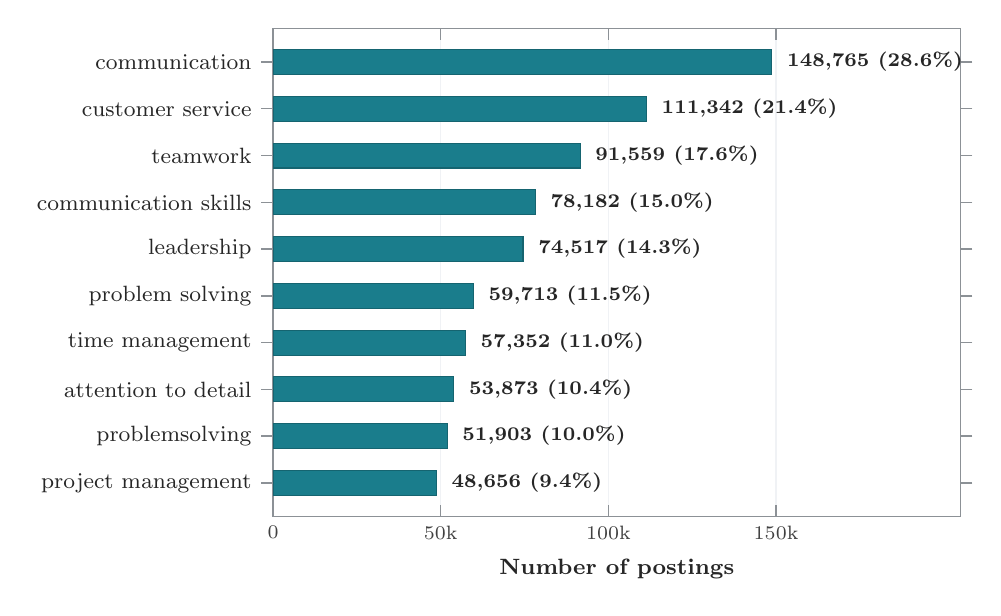
\begin{tikzpicture}
\begin{axis}[
  sg axis,
  xbar,
  bar width=9pt,
  width=0.72\linewidth,
  height=6.2cm,
  symbolic y coords={
    project management,
    problemsolving,
    attention to detail,
    time management,
    problem solving,
    leadership,
    communication skills,
    teamwork,
    customer service,
    communication%
  },
  ytick=data,
  y tick label style={font=\footnotesize, text=black!85, anchor=east},
  xmin=0, xmax=205000,
  xlabel={\textbf{Number of postings}},
  scaled x ticks=false,
  xtick={0,50000,100000,150000},
  xticklabels={0,50k,100k,150k},
  xmajorgrids=true,
  ymajorgrids=false,
  enlarge y limits=0.08,
  nodes near coords,
  nodes near coords align={horizontal},
  every node near coord/.append style={
    font=\scriptsize\bfseries,
    color=black!85,
    anchor=west,
    xshift=2pt
  },
  point meta=explicit symbolic,
]
\addplot[fill=sgTeal, draw=sgTeal!80!black, line width=0.4pt] coordinates {
  (48656,project management) [48,656 (9.4\%)]
  (51903,problemsolving) [51,903 (10.0\%)]
  (53873,attention to detail) [53,873 (10.4\%)]
  (57352,time management) [57,352 (11.0\%)]
  (59713,problem solving) [59,713 (11.5\%)]
  (74517,leadership) [74,517 (14.3\%)]
  (78182,communication skills) [78,182 (15.0\%)]
  (91559,teamwork) [91,559 (17.6\%)]
  (111342,customer service) [111,342 (21.4\%)]
  (148765,communication) [148,765 (28.6\%)]
};
\end{axis}
\end{tikzpicture}%
}%
}

% ============================================================
% FIG 2 — Domain demand / coverage / deficit (ALIGN03)
% ============================================================
\newcommand{\FigGapDemand}{%
\resizebox{\linewidth}{!}{%
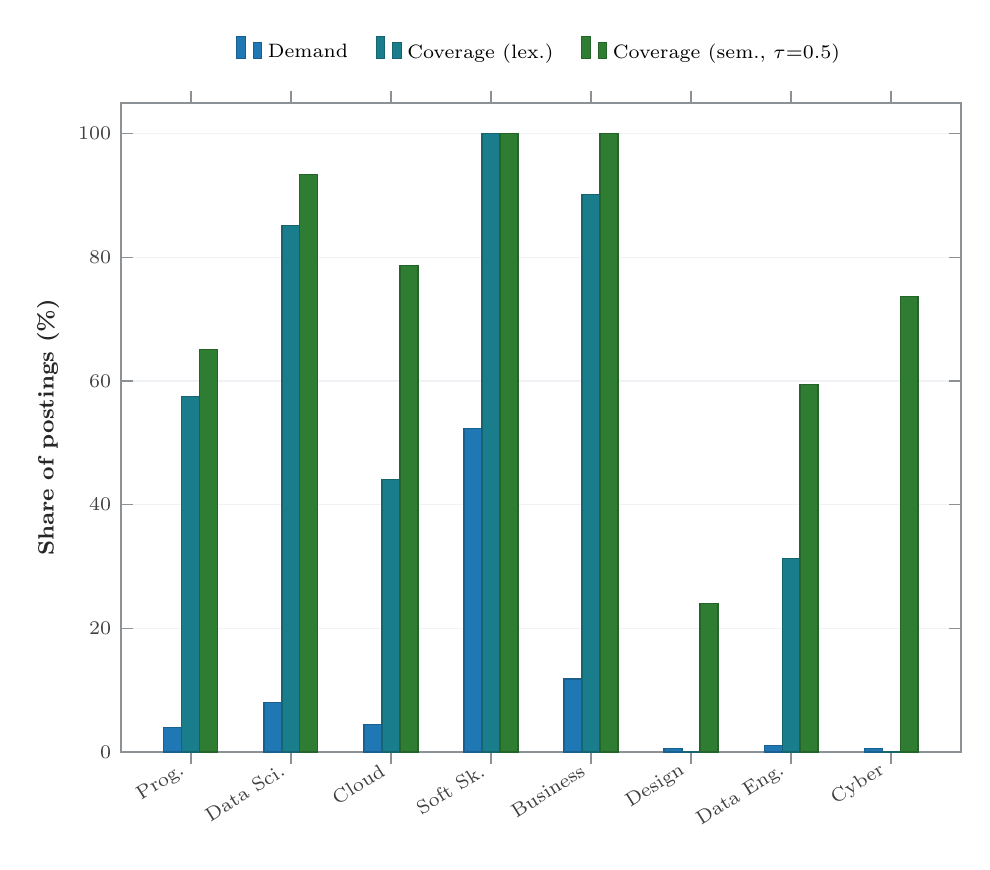
\begin{tikzpicture}
\begin{axis}[
  sg axis,
  ybar,
  bar width=6.5pt,
  width=0.88\linewidth,
  height=0.68\linewidth,
  symbolic x coords={Prog,DataSci,Cloud,Soft,Bus,Design,DataEng,Cyber},
  xtick=data,
  xticklabels={Prog., Data Sci., Cloud, Soft Sk., Business, Design, Data Eng., Cyber},
  x tick label style={rotate=32, anchor=east, font=\scriptsize},
  enlarge x limits=0.10,
  ymin=0, ymax=105,
  ytick={0,20,40,60,80,100},
  ylabel={\textbf{Share of postings (\%)}},
  legend style={
    at={(0.5, 1.04)},
    anchor=south,
    legend columns=-1,
    font=\scriptsize,
    draw=none,
    fill=none,
    /tikz/every even column/.append style={column sep=8pt},
  },
]
\addplot[fill=sgBlue, draw=sgBlue!80!black, line width=0.4pt, bar shift=-6.5pt] coordinates {
  (Prog,3.97)(DataSci,8.04)(Cloud,4.39)(Soft,52.26)(Bus,11.81)(Design,0.60)(DataEng,1.02)(Cyber,0.62)
};
\addlegendentry{Demand}
\addplot[fill=sgTeal, draw=sgTeal!80!black, line width=0.4pt, bar shift=0pt] coordinates {
  (Prog,57.47)(DataSci,85.10)(Cloud,44.06)(Soft,100)(Bus,90.22)(Design,0)(DataEng,31.28)(Cyber,0)
};
\addlegendentry{Coverage (lex.)}
\addplot[fill=sgGreen, draw=sgGreen!80!black, line width=0.4pt, bar shift=6.5pt] coordinates {
  (Prog,65.05)(DataSci,93.36)(Cloud,78.67)(Soft,100)(Bus,100)(Design,24.07)(DataEng,59.50)(Cyber,73.71)
};
\addlegendentry{Coverage (sem., $\tau{=}0.5$)}
\end{axis}
\end{tikzpicture}%
}%
}

\newcommand{\FigGapDeficit}{%
\resizebox{\linewidth}{!}{%
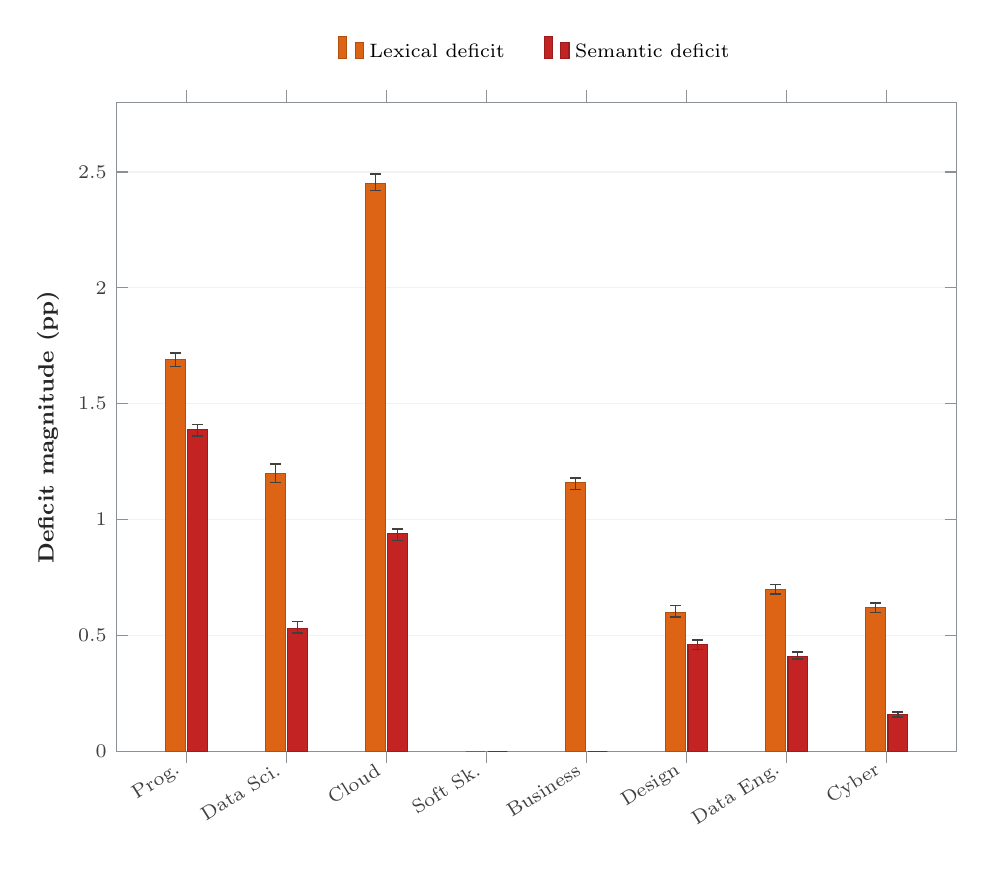
\begin{tikzpicture}
\begin{axis}[
  sg axis,
  ybar,
  bar width=7pt,
  width=0.88\linewidth,
  height=0.68\linewidth,
  symbolic x coords={Prog,DataSci,Cloud,Soft,Bus,Design,DataEng,Cyber},
  xtick=data,
  xticklabels={Prog., Data Sci., Cloud, Soft Sk., Business, Design, Data Eng., Cyber},
  x tick label style={rotate=32, anchor=east, font=\scriptsize},
  enlarge x limits=0.10,
  ymin=0, ymax=2.8,
  ytick={0,0.5,1.0,1.5,2.0,2.5},
  ylabel={\textbf{Deficit magnitude (pp)}},
  legend style={
    at={(0.5, 1.04)},
    anchor=south,
    legend columns=-1,
    font=\scriptsize,
    draw=none,
    fill=none,
    /tikz/every even column/.append style={column sep=12pt},
  },
]
\addplot[fill=sgOrange, draw=sgOrange!80!black, line width=0.4pt, bar shift=-4pt] coordinates {
  (Prog,1.69)(DataSci,1.20)(Cloud,2.45)(Soft,0.00)(Bus,1.16)(Design,0.60)(DataEng,0.70)(Cyber,0.62)
};
\addlegendentry{Lexical deficit}
\addplot[fill=sgRed, draw=sgRed!80!black, line width=0.4pt, bar shift=4pt] coordinates {
  (Prog,1.39)(DataSci,0.53)(Cloud,0.94)(Soft,0.00)(Bus,0.00)(Design,0.46)(DataEng,0.41)(Cyber,0.16)
};
\addlegendentry{Semantic deficit}

% Exact 95% bootstrap CI on Lexical deficit (shifted -4pt)
\draw[black!75, line width=0.6pt] ([xshift=-4pt]axis cs:Prog,1.66) -- ([xshift=-4pt]axis cs:Prog,1.72);
\draw[black!75, line width=0.6pt] ([xshift=-6pt]axis cs:Prog,1.66) -- ([xshift=-2pt]axis cs:Prog,1.66);
\draw[black!75, line width=0.6pt] ([xshift=-6pt]axis cs:Prog,1.72) -- ([xshift=-2pt]axis cs:Prog,1.72);

\draw[black!75, line width=0.6pt] ([xshift=-4pt]axis cs:DataSci,1.16) -- ([xshift=-4pt]axis cs:DataSci,1.24);
\draw[black!75, line width=0.6pt] ([xshift=-6pt]axis cs:DataSci,1.16) -- ([xshift=-2pt]axis cs:DataSci,1.16);
\draw[black!75, line width=0.6pt] ([xshift=-6pt]axis cs:DataSci,1.24) -- ([xshift=-2pt]axis cs:DataSci,1.24);

\draw[black!75, line width=0.6pt] ([xshift=-4pt]axis cs:Cloud,2.42) -- ([xshift=-4pt]axis cs:Cloud,2.49);
\draw[black!75, line width=0.6pt] ([xshift=-6pt]axis cs:Cloud,2.42) -- ([xshift=-2pt]axis cs:Cloud,2.42);
\draw[black!75, line width=0.6pt] ([xshift=-6pt]axis cs:Cloud,2.49) -- ([xshift=-2pt]axis cs:Cloud,2.49);

\draw[black!75, line width=0.6pt] ([xshift=-4pt]axis cs:Bus,1.13) -- ([xshift=-4pt]axis cs:Bus,1.18);
\draw[black!75, line width=0.6pt] ([xshift=-6pt]axis cs:Bus,1.13) -- ([xshift=-2pt]axis cs:Bus,1.13);
\draw[black!75, line width=0.6pt] ([xshift=-6pt]axis cs:Bus,1.18) -- ([xshift=-2pt]axis cs:Bus,1.18);

\draw[black!75, line width=0.6pt] ([xshift=-4pt]axis cs:Design,0.58) -- ([xshift=-4pt]axis cs:Design,0.63);
\draw[black!75, line width=0.6pt] ([xshift=-6pt]axis cs:Design,0.58) -- ([xshift=-2pt]axis cs:Design,0.58);
\draw[black!75, line width=0.6pt] ([xshift=-6pt]axis cs:Design,0.63) -- ([xshift=-2pt]axis cs:Design,0.63);

\draw[black!75, line width=0.6pt] ([xshift=-4pt]axis cs:DataEng,0.68) -- ([xshift=-4pt]axis cs:DataEng,0.72);
\draw[black!75, line width=0.6pt] ([xshift=-6pt]axis cs:DataEng,0.68) -- ([xshift=-2pt]axis cs:DataEng,0.68);
\draw[black!75, line width=0.6pt] ([xshift=-6pt]axis cs:DataEng,0.72) -- ([xshift=-2pt]axis cs:DataEng,0.72);

\draw[black!75, line width=0.6pt] ([xshift=-4pt]axis cs:Cyber,0.60) -- ([xshift=-4pt]axis cs:Cyber,0.64);
\draw[black!75, line width=0.6pt] ([xshift=-6pt]axis cs:Cyber,0.60) -- ([xshift=-2pt]axis cs:Cyber,0.60);
\draw[black!75, line width=0.6pt] ([xshift=-6pt]axis cs:Cyber,0.64) -- ([xshift=-2pt]axis cs:Cyber,0.64);

% Exact 95% bootstrap CI on Semantic deficit (shifted +4pt)
\draw[black!75, line width=0.6pt] ([xshift=4pt]axis cs:Prog,1.36) -- ([xshift=4pt]axis cs:Prog,1.41);
\draw[black!75, line width=0.6pt] ([xshift=2pt]axis cs:Prog,1.36) -- ([xshift=6pt]axis cs:Prog,1.36);
\draw[black!75, line width=0.6pt] ([xshift=2pt]axis cs:Prog,1.41) -- ([xshift=6pt]axis cs:Prog,1.41);

\draw[black!75, line width=0.6pt] ([xshift=4pt]axis cs:DataSci,0.51) -- ([xshift=4pt]axis cs:DataSci,0.56);
\draw[black!75, line width=0.6pt] ([xshift=2pt]axis cs:DataSci,0.51) -- ([xshift=6pt]axis cs:DataSci,0.51);
\draw[black!75, line width=0.6pt] ([xshift=2pt]axis cs:DataSci,0.56) -- ([xshift=6pt]axis cs:DataSci,0.56);

\draw[black!75, line width=0.6pt] ([xshift=4pt]axis cs:Cloud,0.91) -- ([xshift=4pt]axis cs:Cloud,0.96);
\draw[black!75, line width=0.6pt] ([xshift=2pt]axis cs:Cloud,0.91) -- ([xshift=6pt]axis cs:Cloud,0.91);
\draw[black!75, line width=0.6pt] ([xshift=2pt]axis cs:Cloud,0.96) -- ([xshift=6pt]axis cs:Cloud,0.96);

\draw[black!75, line width=0.6pt] ([xshift=4pt]axis cs:Design,0.44) -- ([xshift=4pt]axis cs:Design,0.48);
\draw[black!75, line width=0.6pt] ([xshift=2pt]axis cs:Design,0.44) -- ([xshift=6pt]axis cs:Design,0.44);
\draw[black!75, line width=0.6pt] ([xshift=2pt]axis cs:Design,0.48) -- ([xshift=6pt]axis cs:Design,0.48);

\draw[black!75, line width=0.6pt] ([xshift=4pt]axis cs:DataEng,0.40) -- ([xshift=4pt]axis cs:DataEng,0.43);
\draw[black!75, line width=0.6pt] ([xshift=2pt]axis cs:DataEng,0.40) -- ([xshift=6pt]axis cs:DataEng,0.40);
\draw[black!75, line width=0.6pt] ([xshift=2pt]axis cs:DataEng,0.43) -- ([xshift=6pt]axis cs:DataEng,0.43);

\draw[black!75, line width=0.6pt] ([xshift=4pt]axis cs:Cyber,0.15) -- ([xshift=4pt]axis cs:Cyber,0.17);
\draw[black!75, line width=0.6pt] ([xshift=2pt]axis cs:Cyber,0.15) -- ([xshift=6pt]axis cs:Cyber,0.15);
\draw[black!75, line width=0.6pt] ([xshift=2pt]axis cs:Cyber,0.17) -- ([xshift=6pt]axis cs:Cyber,0.17);

\end{axis}
\end{tikzpicture}%
}%
}

% ============================================================
% FIG 3a — Geographic shares (GEO01)
% ============================================================
\newcommand{\FigGeo}{%
\resizebox{0.95\linewidth}{!}{%
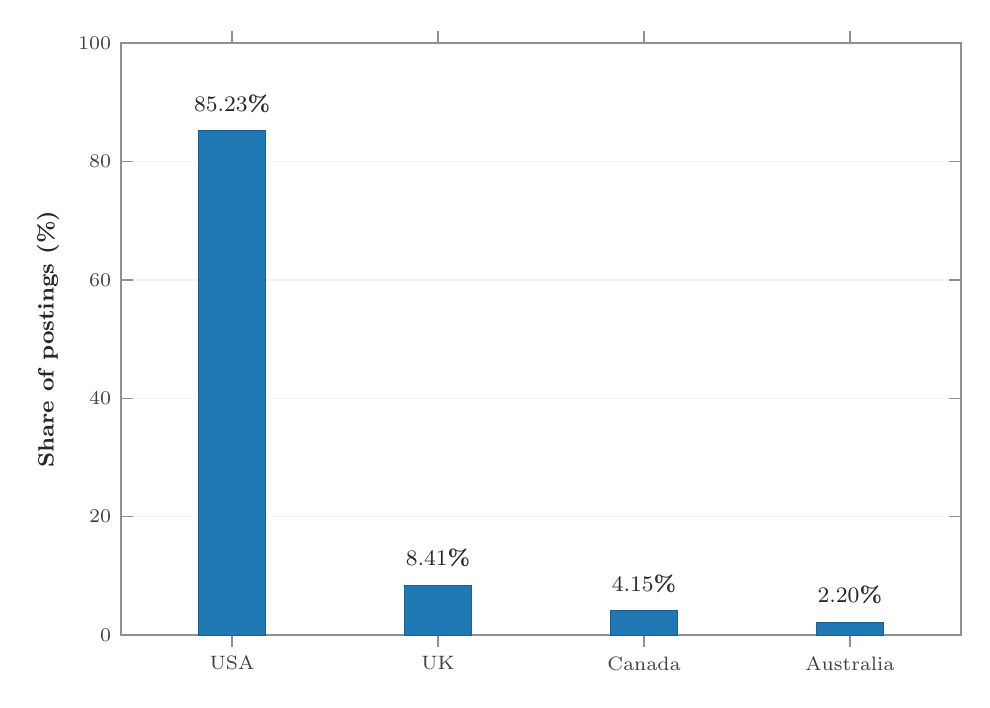
\begin{tikzpicture}
\begin{axis}[
  sg axis,
  ybar,
  bar width=24pt,
  width=0.88\linewidth,
  height=0.62\linewidth,
  symbolic x coords={USA,UK,Canada,Australia},
  xtick=data,
  ymin=0, ymax=100,
  ylabel={\textbf{Share of postings (\%)}},
  enlarge x limits=0.18,
  nodes near coords={\pgfmathprintnumber[fixed, zerofill=true, precision=2]{\pgfplotspointmeta}\%},
  every node near coord/.append style={font=\footnotesize\bfseries, color=black!85, yshift=3pt},
]
\addplot[sg bar=sgBlue] coordinates {
  (USA,85.23)(UK,8.41)(Canada,4.15)(Australia,2.20)
};
\end{axis}
\end{tikzpicture}%
}%
}

% ============================================================
% FIG 4a — Cohen's d (STAT01)
% ============================================================
\newcommand{\FigEffectSizes}{%
\resizebox{\linewidth}{!}{%
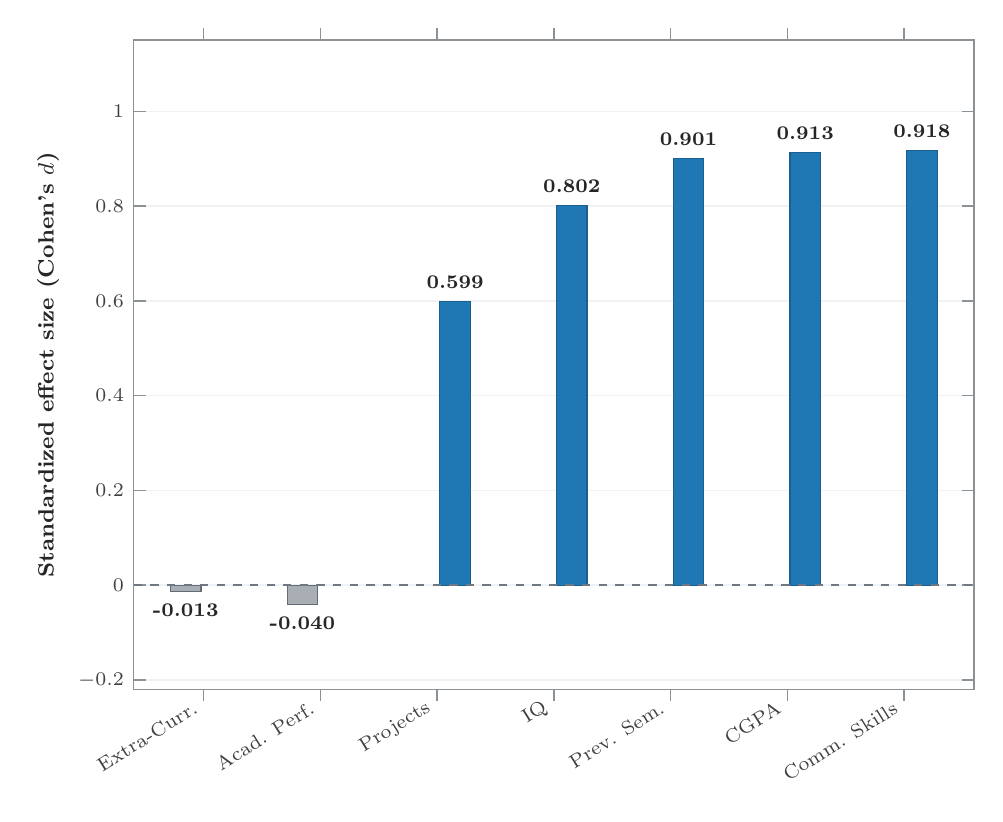
\begin{tikzpicture}
\begin{axis}[
  sg axis,
  ybar,
  bar width=11pt,
  width=0.88\linewidth,
  height=0.68\linewidth,
  symbolic x coords={ExtraCurr,AcadPerf,Projects,IQ,PrevSem,CGPA,CommSk},
  xtick={ExtraCurr,AcadPerf,Projects,IQ,PrevSem,CGPA,CommSk},
  xticklabels={Extra-Curr., Acad. Perf., Projects, IQ, Prev. Sem., CGPA, Comm. Skills},
  x tick label style={rotate=32, anchor=east, font=\scriptsize},
  ymin=-0.22, ymax=1.15,
  ylabel={\textbf{Standardized effect size (Cohen's $d$)}},
  enlarge x limits=0.10,
  point meta=explicit symbolic,
  nodes near coords,
]
\addplot[fill=sgGrey!60, draw=sgGrey!90!black, line width=0.4pt, every node near coord/.append style={font=\scriptsize\bfseries, color=black!85, anchor=north, yshift=-1pt}] coordinates {
  (ExtraCurr,-0.013) [-0.013]
  (AcadPerf,-0.040) [-0.040]
};
\addplot[fill=sgBlue, draw=sgBlue!80!black, line width=0.4pt, every node near coord/.append style={font=\scriptsize\bfseries, color=black!85, anchor=south, yshift=1pt}] coordinates {
  (Projects,0.599) [0.599]
  (IQ,0.802) [0.802]
  (PrevSem,0.901) [0.901]
  (CGPA,0.913) [0.913]
  (CommSk,0.918) [0.918]
};
\draw[dashed, sgGrey, line width=0.5pt] ({axis cs:ExtraCurr,0} -| {rel axis cs:0,0}) -- ({rel axis cs:1,0} |- {axis cs:ExtraCurr,0});
\end{axis}
\end{tikzpicture}%
}%
}

% ============================================================
% FIG 4b — Group means (STAT01)
% ============================================================
\newcommand{\FigMeans}{%
\resizebox{\linewidth}{!}{%
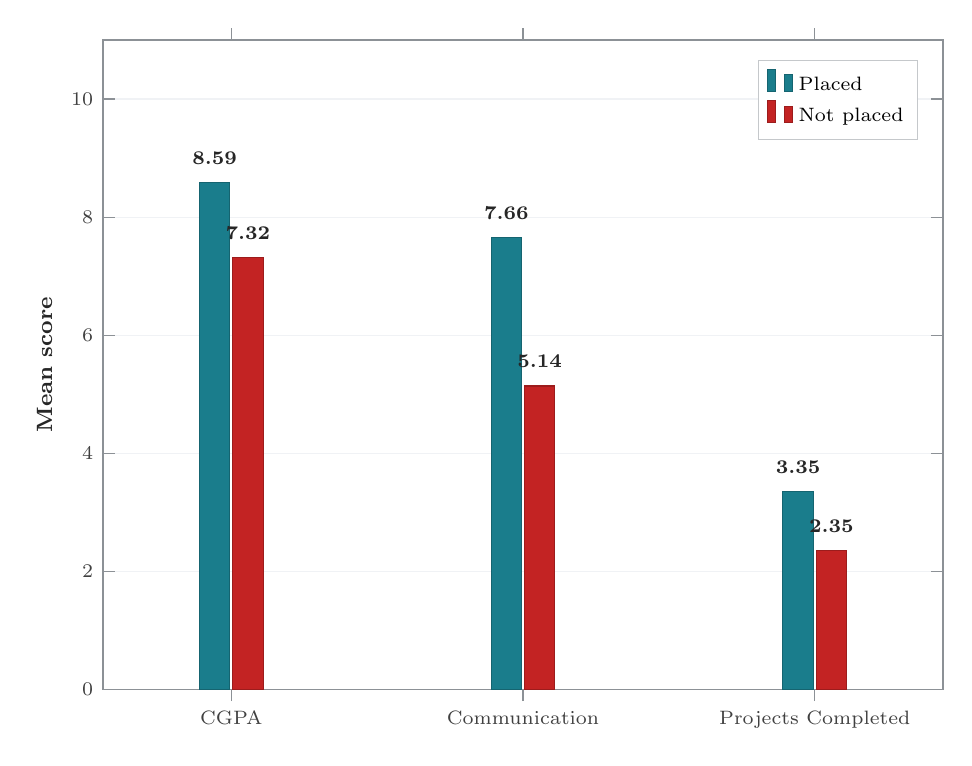
\begin{tikzpicture}
\begin{axis}[
  sg axis,
  ybar,
  bar width=11pt,
  width=0.88\linewidth,
  height=0.68\linewidth,
  symbolic x coords={CGPA,Comm,Projects},
  xtick=data,
  xticklabels={CGPA, Communication, Projects Completed},
  x tick label style={font=\scriptsize},
  ymin=0, ymax=11.0,
  ylabel={\textbf{Mean score}},
  enlarge x limits=0.22,
  legend pos=north east,
  point meta=explicit symbolic,
  nodes near coords,
  every node near coord/.append style={font=\scriptsize\bfseries, color=black!85, yshift=3pt},
]
\addplot[fill=sgTeal, draw=sgTeal!80!black, line width=0.4pt, bar shift=-6pt] coordinates {
  (CGPA,8.59) [8.59]
  (Comm,7.66) [7.66]
  (Projects,3.35) [3.35]
};
\addlegendentry{Placed}
\addplot[fill=sgRed, draw=sgRed!80!black, line width=0.4pt, bar shift=6pt] coordinates {
  (CGPA,7.32) [7.32]
  (Comm,5.14) [5.14]
  (Projects,2.35) [2.35]
};
\addlegendentry{Not placed}
\end{axis}
\end{tikzpicture}%
}%
}

% ============================================================
% FIG 5 — Internship employment rates (INTL01)
% ============================================================
\newcommand{\FigInternship}{%
\resizebox{0.88\linewidth}{!}{%
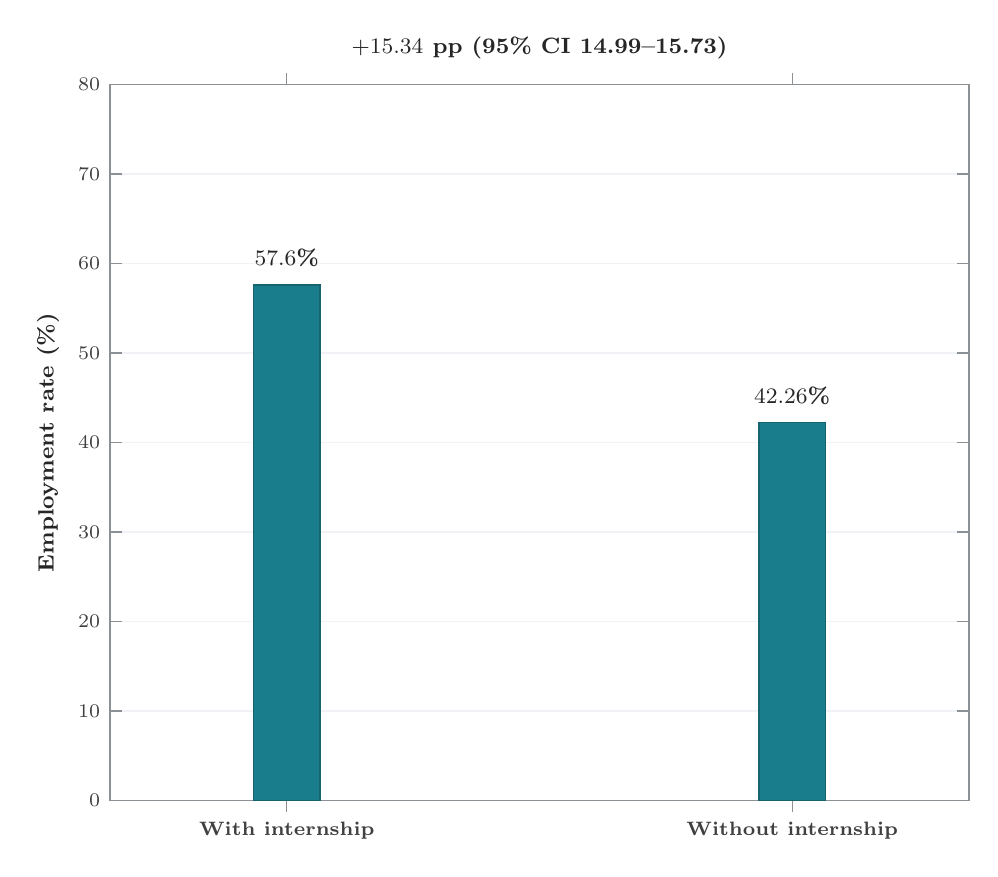
\begin{tikzpicture}
\begin{axis}[
  sg axis,
  ybar,
  bar width=24pt,
  width=0.90\linewidth,
  height=0.75\linewidth,
  symbolic x coords={With,Without},
  xtick={With,Without},
  xticklabels={With internship, Without internship},
  x tick label style={font=\scriptsize\bfseries},
  ymin=0, ymax=80,
  ylabel={\textbf{Employment rate (\%)}},
  enlarge x limits=0.35,
  nodes near coords={\pgfmathprintnumber[fixed, precision=2]{\pgfplotspointmeta}\%},
  every node near coord/.append style={font=\footnotesize\bfseries, color=black!85, yshift=3pt},
]
\addplot[fill=sgTeal, draw=sgTeal!80!black, line width=0.4pt] coordinates {
  (With,57.60)(Without,42.26)
};
\end{axis}
\node[font=\footnotesize\bfseries, text=black!85, anchor=south, align=center]
  at (current axis.north) [yshift=2mm]
  {$+15.34$ pp (95\% CI 14.99--15.73)};
\end{tikzpicture}%
}%
}

\setlength{\parskip}{0pt}
\setlength{\parindent}{1em}

% Hyperref setup
\hypersetup{
    colorlinks=true,
    linkcolor=blue,
    filecolor=magenta,
    urlcolor=cyan,
    citecolor=blue,
}

% Double-blind anonymity: strip the build timestamp (it embeds the build
% machine's timezone) and the producer/creator identification strings from the
% PDF trailer.  These are pdfTeX primitives; harmless if ignored by a
% different engine.
\pdfinfoomitdate=1
\pdfsuppressptexinfo=-1
\pdftrailerid{}

% Paper Title
\title{A Benchmark Audit of Graduate-Placement Modeling: Decision Boundaries, External Cohorts, and the Limits of Near-Perfect Placement Scores}

\author{
\IEEEauthorblockN{Author Names Redacted for Double-Blind Peer Review}\\
\IEEEauthorblockA{\textit{Department of Computer Science and Engineering}\\
Academic Research Institution\\
contact@university.edu}
\thanks{Companion article to ``Lexical versus Semantic Skill-Gap Measurement: A Sensitivity Audit on Job-Posting Data'' (gap-measurement paper). Manuscript submitted for peer review.}
}

\begin{document}

\maketitle

% ============================================================
% ABSTRACT
% ============================================================
\begin{abstract}
Near-perfect classification scores on graduate-placement benchmarks are routinely read as evidence about employability. This companion article re-examines the placement component of an academic--industry skill-gap study as a \textit{benchmark audit}. Every cohort involved---College Student Placement ($N = 10{,}000$), Global Student Placement ($N = 10{,}000$), Student Career Success ($N = 50{,}000$), and International Graduates ($N = 300{,}000$)---carries generator-signature evidence over an unverified provenance record (a fifth file, India Skills Intelligence, declares itself synthetic in its source README), so the four registered placement experiments (STAT01, STAT02, PLAC01, INTL01) are treated as audits of benchmark behaviour, and we draw no conclusions about real graduates. The audit establishes four facts. First, the college benchmark's placement label is a deterministic $k$-of-$n$ threshold rule (three of four conditions; 99.92\% of label assignments), which tree ensembles reproduce at 99.99\% accuracy while a linear model reaches 90.11\% (ROC-AUC 0.9406). Second, transferring that model to distinct external benchmark cohorts degrades discrimination to ROC-AUC 0.768 and 0.576: near-perfect in-distribution scores measure decision-boundary recovery, not generalizable predictability. Third, cross-country placement rates in the global benchmark span only 3.18 percentage points with overlapping 95\% confidence intervals, which---because that benchmark's provenance is unverified (moderate generator signatures)---leaves the credential-locality hypothesis (H5) \textit{untested} rather than refuted. Fourth, the registered internship hypothesis (H6) is not supported within the benchmark (univariate risk difference $-0.44$ pp; odds ratio $1.02$, $p = 0.62$), while the signaling ordering (H4) is reproduced by construction. The international-graduate internship contrast (INTL01) is retained as an archived artifact but is reported as no finding: an effect estimate on a generated file cannot be attributed to graduates (the effect size itself is deliberately not printed in either article). We recommend that benchmark-based employability studies report provenance flags, decision-boundary diagnostics, and external-cohort evaluation as standard practice.
\end{abstract}

\begin{IEEEkeywords}
Graduate placement, Benchmark audit, Decision boundaries, Cross-validation, External validity, Benchmark provenance tiers, Employability modeling.
\end{IEEEkeywords}

% ============================================================
% SECTION 1: INTRODUCTION
% ============================================================
\section{Introduction}
\label{sec:intro_p}

Predictive models of graduate placement now routinely report cross-validated accuracies in the high nineties, and such scores are frequently interpreted as findings about which academic and behavioral traits drive employability. The audit reported here asks a narrower, methodological question: \textit{what do these scores actually measure, given what the underlying data are?} We answer it for the four registered placement experiments of a larger academic--industry skill-gap study whose gap-measurement results (hypotheses H1--H3 on posting corpora) are reported in the companion article.

The first step is provenance. A generator-signature audit of every benchmark file in the project (\texttt{datasets/REAL\_VS\_SYNTHETIC.csv}; executable checks in \texttt{datasets/synthetic\_checks.py} with outputs in \texttt{datasets/synthetic\_checks\_output.json}) assigns the College Placement and Global Placement files a \textit{moderate generator-signature} tier, International Graduates a \textit{weak/partial} tier, and Student Career Success \textit{no generator signatures found}, over provenance records that no source documents: sequential identifiers, uniform-consistent categorical draws, balanced pseudo-longitudinal fields, and deterministic label rules are present in several of them, and no source states a collection protocol for real graduates. One further file, India Skills Intelligence, is declared synthetic by its own README. No real graduate records are involved anywhere in this article.

Given that provenance, this article makes four contributions:
\begin{enumerate}
    \item \textbf{A boundary audit:} We show that the college benchmark's placement label is generated by a deterministic $k$-of-$n$ threshold rule (three of four conditions account for 99.92\% of assignments) and that tree ensembles---whose axis-parallel partitions align with such step functions---accordingly score 99.99\%/99.97\%, while logistic regression reaches 90.11\% (ROC-AUC 0.9406).
    \item \textbf{An external-cohort transfer audit:} The same model degrades to ROC-AUC 0.768 and 0.576 on distinct external benchmark cohorts (in-sample references: 0.782/0.714), demonstrating that near-perfect in-distribution scores reflect benchmark-specific rules rather than transferable predictability.
    \item \textbf{Reframed hypothesis verdicts:} H4 (signaling hierarchy), H5 (credential locality), and H6 (internship returns) are reported strictly as properties of benchmarks with unverified, tier-flagged provenance. H5 is left \textit{untested}, and the INTL01 internship contrast is deliberately not reported as a finding.
    \item \textbf{Reporting recommendations:} We argue that provenance flags, decision-boundary diagnostics, and external-cohort evaluation should be standard reporting practice for benchmark-based employability studies.
\end{enumerate}

The remainder of this article is organized as follows: Section~\ref{sec:related_p} reviews the employability-modeling literature and the theory behind hypotheses H4--H6. Section~\ref{sec:methodology_p} documents the benchmark files and the statistical and predictive protocols. Section~\ref{sec:results_p} presents the audit. Section~\ref{sec:discussion_p} gives verdicts, recommendations, reproducibility, and threats to validity. Section~\ref{sec:conclusion_p} concludes.

% ============================================================
% SECTION 2: RELATED WORK AND HYPOTHESES
% ============================================================
\section{Related Work and Theoretical Foundations}
\label{sec:related_p}

\subsection{Machine Learning in Employability Modeling}

Predictive modeling of graduate placement has expanded from discriminant analysis to ensemble learning. Tree-based ensembles such as Random Forests and Gradient Boosting frequently yield higher cross-validated accuracy than linear models in educational placement benchmarks \cite{tamene2024predictive, haque2024classification}. Feature-importance analyses in these studies typically identify academic performance and project engagement as leading predictors. However, benchmark evaluations in this literature often report high classification accuracy without assessing decision-boundary structure, multicollinearity, or performance on independent external cohorts. This article supplies exactly those three missing audits.

\subsection{Theoretical Grounding of H4--H6}
\label{sec:theory_p}

Two of the companion article's four theoretical perspectives bear directly on the placement hypotheses:

\textbf{1) Human Capital Theory (HCT):} Formulated by Becker \cite{becker1964human} and Schultz \cite{schultz1961investment}, HCT posits that education enhances productive capacity, yielding labor-market returns. HCT distinguishes between \textit{general human capital} (transferable competencies such as critical thinking, communication, and core mathematical reasoning) and \textit{firm-specific human capital} (proficiency with specialized software tools, proprietary APIs, or operational frameworks). Internship participation is conventionally read as firm-specific accumulation---the reading hypothesis H6 tests.

\textbf{2) Job Market Signaling and Screening Theory:} Spence \cite{spence1973job} established that in labor markets characterized by asymmetric information, employers cannot directly observe an applicant's innate productivity prior to hiring. Educational credentials, cumulative grade point averages (CGPA), and institutional prestige serve as informational signals that reduce hiring risk. In technical recruitment, however, degree credentials are increasingly complemented by practical capability signals, such as project portfolios, open-source contributions, and technical internship certifications \cite{pianda2024impact, scandurra2024employability}.

\subsection{Hypotheses H4--H6 (Restated)}
\label{sec:hypotheses_p}

The companion article derives six hypotheses from four theoretical perspectives; its gap-measurement hypotheses H1--H3 concern posting corpora and are reported there. The three placement hypotheses are restated below, with their verdicts evaluated strictly as \textit{benchmark properties}:
\begin{enumerate}[label=\textbf{H\arabic*:}, start=4]
    \item \textbf{Signaling hierarchy:} Under job-market signaling \cite{spence1973job}, legible capability signals---communication proficiency, completed projects, and cumulative academic performance---should dominate placement odds after mutual statistical control. \textit{Test:} STAT01 multivariate logistic regression.
    \item \textbf{Credential locality:} If credentials function as locally interpreted signals, placement rates should differ systematically across national labor markets. \textit{Test:} PLAC01 cross-country placement-rate comparison ($N = 10{,}000$).
    \item \textbf{Human-capital returns to internships:} If internship participation constitutes firm-specific human-capital accumulation \cite{becker1964human}, internship experience should predict placement even after controls. \textit{Test:} STAT01 college-cohort internship risk difference and multivariate odds ratio, with INTL01 as an external descriptive check on a separate international-graduate benchmark of unverified provenance (a pre-registered null remains informative: participation \textit{per se}, unlike communication skill or project evidence, may be too coarse a signal).
\end{enumerate}

% ============================================================
% SECTION 3: METHODOLOGY
% ============================================================
\section{Methodology}
\label{sec:methodology_p}

\subsection{Benchmarks and Provenance}
\label{sec:corpus_p}

The audit uses four tabular benchmarks, all acquired from public benchmark repositories in September 2026: College Student Placement ($N = 10{,}000$; 1,659 placed) \cite{sumedh15072024college}, Global Student Placement ($N = 10{,}000$) \cite{rakesh6302024global}, Student Career Success ($N = 50{,}000$) \cite{mobeenfatimah2024career}, and International Graduates ($N = 300{,}000$) \cite{quackquackrp2024international}. Every one of the four carries an unverified provenance record with generator signatures in the moderate (College Placement, Global Placement) or weak/partial (International Graduates) tiers, while Student Career Success shows no discriminating generator signature at all (sequential zero-padded identifiers, uniform-consistent categorical draws, deterministic label rules are present in the flagged files), and no source documents collection of real graduate records (\texttt{datasets/REAL\_VS\_SYNTHETIC.csv}; \texttt{datasets/synthetic\_checks\_output.json}). They contain academic, behavioral, and placement indicators---no personally identifying information, and no real graduates. All quantities in this article are therefore properties of these benchmark files. Where a verdict would ordinarily be stated about graduates, we state it about the benchmark instead, or decline to state it (H5).

\subsection{Statistical Inference \& Collinearity Diagnostics}

Differences between placed and non-placed students are tested using Welch's $t$-test (accounting for unequal variances):
\begin{equation}
t = \frac{\bar{X}_1 - \bar{X}_2}{\sqrt{\frac{s_1^2}{n_1} + \frac{s_2^2}{n_2}}}
\label{eq:welch}
\end{equation}
Standardized effect sizes are quantified via Cohen's $d$:
\begin{equation}
d = \frac{\bar{X}_1 - \bar{X}_2}{s_{\text{pooled}}}, \quad s_{\text{pooled}} = \sqrt{\frac{(n_1-1)s_1^2 + (n_2-1)s_2^2}{n_1 + n_2 - 2}}
\label{eq:cohen}
\end{equation}

Categorical dependencies are evaluated using the Chi-square statistic $\chi^2$ and Cram\'er's $V$:
\begin{equation}
V = \sqrt{\frac{\chi^2}{n \cdot \min(r-1, c-1)}}
\label{eq:cramer}
\end{equation}

Multicollinearity among continuous predictors $\mathbf{X}$ is assessed with Variance Inflation Factors (VIF). For standardized feature matrices, the VIF vector is obtained from the diagonal of the inverted correlation matrix:
\begin{equation}
\text{VIF}_j = \left(\mathbf{R}^{-1}\right)_{jj} = \frac{1}{1 - R_j^2}
\label{eq:vif}
\end{equation}
Features exhibiting $\text{VIF}_j > 5.0$ are flagged as collinear.

\subsection{Predictive Modeling \& Validation Protocols}

Graduate placement prediction is evaluated as a binary classification task: predicting outcome $y \in \{0, 1\}$ ($1 = \text{Placed}$, $0 = \text{Not Placed}$) given student feature vector $\mathbf{x} = [\text{CGPA}, \text{Comm}, \text{Projects}, \text{Internship}, \text{IQ}, \text{AcademicPerf}]^T$. Continuous features are standardized to zero mean and unit variance within training partitions:
\begin{equation}
z_{ij} = \frac{x_{ij} - \mu_j}{\sigma_j}
\label{eq:standardize}
\end{equation}

In the standardized logistic regression model:
\begin{equation}
\ln\left(\frac{P(y=1|\mathbf{z})}{1 - P(y=1|\mathbf{z})}\right) = \beta_0 + \sum_{j=1}^p \beta_j z_j
\label{eq:logistic}
\end{equation}
The odds ratio $\text{OR}_j = \exp(\beta_j)$ represents the change in odds associated with a one-standard-deviation increase in predictor $j$.

Model performance is evaluated using 5-fold stratified cross-validation ($\text{random\_state} = 42$) across five classifier paradigms:
\begin{enumerate}
    \item \textbf{Logistic Regression:} $\ell_2$-regularized, $C = 1.0$, solved via L-BFGS.
    \item \textbf{Random Forest:} $B = 100$ estimators, maximum tree depth $= 12$, Gini split criterion.
    \item \textbf{Support Vector Machine (SVM):} Radial Basis Function (RBF) kernel, $C = 1.0$, $\gamma = \text{scale}$, with Platt probability calibration.
    \item \textbf{Decision Tree:} Single CART tree with maximum depth $= 6$.
    \item \textbf{Majority-Class Baseline:} Classifier predicting the empirical majority class.
\end{enumerate}

To evaluate model behavior under domain shift, we train the standardized logistic regression model on the College Placement benchmark ($N = 10,000$) and evaluate it on a held-out Student Career Success benchmark ($N = 50,000$; provenance unverified, no generator signatures found) using domain-standardized continuous predictors.

% ============================================================
% SECTION 4: RESULTS
% ============================================================
\section{Benchmark Audit Results}
\label{sec:results_p}

\subsection{RQ4: Employability Determinants \& Cross-Validation Benchmarks}

All statistics in this subsection describe model behaviour on benchmarks with unverified provenance (Section~\ref{sec:corpus_p}); none of them is evidence about real graduates.

\subsubsection{Univariate \& Descriptive Findings}
In the College Placement cohort ($N = 10,000$; 1,659 placed, 8,341 not placed, base placement rate $16.59\%$), placed students had higher mean values across key academic and skill indicators (Table~\ref{tab:descriptive}). Placed individuals had higher average CGPA ($8.59 \pm 1.15$ vs. $7.32 \pm 1.44$, $t = 39.37$, $p < 0.001$, Cohen's $d = 0.913$), higher communication scores ($7.66 \pm 2.59$ vs. $5.14 \pm 2.78$, $t = 35.79$, $p < 0.001$, Cohen's $d = 0.918$), and more completed projects ($3.35 \pm 1.28$ vs. $2.35 \pm 1.74$, $t = 27.21$, $p < 0.001$, Cohen's $d = 0.599$). Generalized academic performance ratings ($p = 0.1386$, $d = -0.040$) and extra-curricular participation scores ($p = 0.6383$, $d = -0.013$) showed negligible differences between groups.

\begin{table}[!htbp]
\centering
\caption{Descriptive Statistics: Placed vs. Non-Placed Cohort ($N = 10,000$)}
\label{tab:descriptive}
\resizebox{\columnwidth}{!}{%
% AUTO-GENERATED by experiments/make_latex.py -- do not edit
\begin{tabular}{@{}lccccc@{}}
\toprule
\textbf{Variable} & \textbf{Placed ($n=1659$)} & \textbf{Not Placed ($n=8341$)} & \textbf{$t$-stat} & \textbf{$p$-value} & \textbf{Cohen's $d$} \\
\midrule
CGPA & $8.59 \pm 1.15$ & $7.32 \pm 1.44$ & 39.37 & <0.001 & 0.913 \\
IQ & $109.12 \pm 15.21$ & $97.55 \pm 14.26$ & 28.58 & <0.001 & 0.802 \\
Prev. Sem. Result & $8.57 \pm 1.13$ & $7.33 \pm 1.42$ & 38.96 & <0.001 & 0.901 \\
Comm. Skills & $7.66 \pm 2.59$ & $5.14 \pm 2.78$ & 35.79 & <0.001 & 0.918 \\
Projects & $3.35 \pm 1.28$ & $2.35 \pm 1.74$ & 27.21 & <0.001 & 0.599 \\
Acad. Perf. & $5.45 \pm 2.90$ & $5.57 \pm 2.87$ & -1.48 & 0.1386 & -0.040 \\
Extra-Curr. & $4.94 \pm 3.19$ & $4.98 \pm 3.15$ & -0.47 & 0.6383 & -0.013 \\
\bottomrule
\end{tabular}

}
\end{table}

Bivariate chi-square tests confirm that placement is strongly associated with project completion ($\chi^2(2) = 719.82$, $p < 0.001$, $V = 0.268$) but not with internship experience in this cohort ($\chi^2(1) = 0.31$, $p = 0.578$, $V = 0.006$).

\begin{figure*}[!htbp]
    \centering
    \begin{subfigure}[t]{0.48\textwidth}
        \centering
        \FigEffectSizes
        \caption{Standardized effect sizes (Cohen's $d$)}
        \label{fig:placement_a}
    \end{subfigure}
    \hfill
    \begin{subfigure}[t]{0.48\textwidth}
        \centering
        \FigMeans
        \caption{Group means for key predictors}
        \label{fig:placement_b}
    \end{subfigure}
    \caption{Key predictors for placed versus non-placed students in the college benchmark ($N = 10{,}000$; STAT01). (a) Cohen's $d$ for all seven audited variables; Academic Performance and Extra-Curricular Score are negligible. (b) Group means (all differences in (b) significant at $p < 0.001$, Welch $t$-tests).}
    \label{fig:placement}
\end{figure*}

\subsubsection{Multicollinearity Diagnostics}
Variance Inflation Factors computed for the continuous predictors are summarized in Table~\ref{tab:vif}. All values are $\approx 1.001$ (tolerances $\approx 0.999$), well below the collinearity threshold of 5.0, confirming that multicollinearity does not affect coefficient estimation in this model.

\begin{table}[!htbp]
\centering
\caption{Variance Inflation Factor (VIF) Multicollinearity Audit}
\label{tab:vif}
\resizebox{\columnwidth}{!}{%
% AUTO-GENERATED by experiments/make_latex.py -- do not edit
\begin{tabular}{@{}lccc@{}}
\toprule
\textbf{Feature Name} & \textbf{VIF} & \textbf{Tolerance ($1/\text{VIF}$)} & \textbf{Collinearity Status} \\
\midrule
CGPA & 1.001 & 0.999 & Acceptable ($< 5.0$) \\
Communication Skills & 1.001 & 0.999 & Acceptable ($< 5.0$) \\
Projects Completed & 1.001 & 0.999 & Acceptable ($< 5.0$) \\
Internship Experience & 1.001 & 0.999 & Acceptable ($< 5.0$) \\
IQ & 1.000 & 1.000 & Acceptable ($< 5.0$) \\
Academic Performance & 1.001 & 0.999 & Acceptable ($< 5.0$) \\
\bottomrule
\end{tabular}

}
\end{table}

\subsubsection{Standardized Logistic Regression}
Standardized logistic regression estimates (maximum likelihood with intercept, Wald inference) are reported in Table~\ref{tab:logistic}. A one-standard-deviation increase in Communication Skills is associated with an odds ratio of 6.55 (95\% CI: [5.86, 7.31], $p < 0.001$). CGPA ($\text{OR} = 6.28$, 95\% CI: [5.62, 7.01], $p < 0.001$), IQ score ($\text{OR} = 5.16$, 95\% CI: [4.65, 5.72], $p < 0.001$), and completed projects ($\text{OR} = 3.20$, 95\% CI: [2.92, 3.51], $p < 0.001$) are also positively associated with placement. Neither Internship Experience ($\text{OR} = 1.02$, $p = 0.620$) nor generalized Academic Performance ($\text{OR} = 0.98$, $p = 0.588$) contributes independent signal once the remaining predictors are controlled. Under the audit framing, these coefficients describe which variables the benchmark's label generator encodes---they are not estimates of labor-market effects.

\begin{table}[!htbp]
\centering
\caption{Standardized Logistic Regression Placement Model (STAT01; statsmodels MLE with intercept)}
\label{tab:logistic}
\resizebox{\columnwidth}{!}{%
% AUTO-GENERATED by experiments/make_latex.py -- do not edit
\begin{tabular}{@{}lcccc@{}}
\toprule
\textbf{Predictor Feature} & \textbf{Coef ($\beta$)} & \textbf{Odds Ratio (OR)} & \textbf{95\% CI} & \textbf{$p$-value} \\
\midrule
CGPA & 1.8368 & 6.2765 & [5.62, 7.01] & <0.001 \\
Communication Skills & 1.8790 & 6.5471 & [5.86, 7.31] & <0.001 \\
Projects Completed & 1.1644 & 3.2041 & [2.92, 3.51] & <0.001 \\
Internship Experience & 0.0192 & 1.0194 & [0.94, 1.10] & $0.6197$ \\
IQ & 1.6404 & 5.1570 & [4.65, 5.72] & <0.001 \\
Academic Performance & $-0.0207$ & 0.9795 & [0.91, 1.06] & $0.5884$ \\
\bottomrule
\end{tabular}

}
\end{table}

\subsubsection{5-Fold Cross-Validation Model Comparison}
Table~\ref{tab:model_comparison} documents 5-fold stratified cross-validation performance across five classifier paradigms (mean $\pm$ SD across the five folds, seed 42).

\begin{table}[!htbp]
\centering
\caption{Stratified 5-Fold Cross-Validation Performance Benchmarks (seed 42)}
\label{tab:model_comparison}
\resizebox{\columnwidth}{!}{%
% AUTO-GENERATED by experiments/make_latex.py -- do not edit
\begin{tabular}{@{}lccc@{}}
\toprule
\textbf{Model Architecture} & \textbf{Accuracy (Mean$\pm$SD)} & \textbf{$F_1$-Score} & \textbf{ROC-AUC} \\
\midrule
Logistic Regression & $90.11\% \pm 0.74\%$ & $0.8966 \pm 0.0078$ & $0.9406 \pm 0.0075$ \\
Random Forest & $99.99\% \pm 0.02\%$ & $0.9999 \pm 0.0002$ & $1.0000 \pm 0.0000$ \\
SVM (RBF) & $95.72\% \pm 0.56\%$ & $0.9565 \pm 0.0058$ & $0.9894 \pm 0.0019$ \\
Decision Tree & $99.97\% \pm 0.07\%$ & $0.9997 \pm 0.0007$ & $0.9998 \pm 0.0004$ \\
Baseline (Majority) & $83.41\% \pm 0.02\%$ & $0.7587 \pm 0.0003$ & $0.5000 \pm 0.0000$ \\
\bottomrule
\end{tabular}

}
\end{table}

Results are stable across random seeds: repeating the full 5-fold protocol over 10 seeds (50 fold evaluations per model; Table~\ref{tab:multiseed}) yields a mean accuracy of $90.12\% \pm 0.04\%$ for logistic regression and $95.76\% \pm 0.07\%$ for the SVM, with tree ensembles remaining at $\ge 99.99\%$.

\begin{table}[!htbp]
\centering
\caption{Multi-Seed Robustness: 10 Seeds $\times$ 5 Folds (STAT01)}
\label{tab:multiseed}
\resizebox{\columnwidth}{!}{%
% AUTO-GENERATED by experiments/make_latex.py -- do not edit
\begin{tabular}{@{}lcccc@{}}
\toprule
\textbf{Model} & \textbf{Seeds} & \textbf{Fold Evals} & \textbf{Accuracy (Mean$\pm$SD)} & \textbf{ROC-AUC} \\
\midrule
Logistic Regression & 10 & 50 & $90.12\% \pm 0.04\%$ & $0.9408 \pm 0.0002$ \\
Random Forest & 10 & 50 & $100.00\% \pm 0.00\%$ & $1.0000 \pm 0.0000$ \\
SVM (RBF) & 10 & 50 & $95.76\% \pm 0.07\%$ & $0.9896 \pm 0.0002$ \\
Decision Tree & 10 & 50 & $100.00\% \pm 0.01\%$ & $0.9999 \pm 0.0003$ \\
Baseline (Majority) & 10 & 50 & $83.41\% \pm 0.00\%$ & $0.5000 \pm 0.0000$ \\
\bottomrule
\end{tabular}

}
\end{table}

\subsubsection{Diagnostic Audit of Tree Ensembles \& External Generalization}
\label{sec:diag}
The near-perfect classification performance of Random Forest ($99.99\%$) and Decision Tree ($99.97\%$) models prompted an inspection of the underlying data-generating process. Fitting a depth-4 CART tree to the placement cohort yielded 100\% training accuracy, indicating that placement labels in this benchmark were generated via a deterministic $k$-of-$n$ threshold rule: individuals are labeled as placed when meeting at least three of four conditions ($\text{CGPA} > 8.01$, $\text{IQ} > 110.5$, $\text{Communication} > 7.50$, $\text{Projects} \ge 2$), accounting for $99.92\%$ of label assignments. Because orthogonal recursive partitioning aligns directly with this axis-parallel step function, tree ensembles reproduce the rule with minimal error. Logistic regression estimates a linear decision surface across these features, yielding $90.11\%$ cross-validated accuracy and an ROC-AUC of 0.9406.

To evaluate performance on a held-out benchmark whose provenance is unverified (no generator signatures found), the logistic regression model was tested on the Student Career Success dataset ($N = 50,000$) using standardized values for CGPA, communication, and project count. On this external cohort, discriminative performance decreased to $\text{ROC-AUC} = 0.768$ (accuracy $= 29.9\%$, $F_1 = 0.235$ at the shifted base rate of $78.08\%$), and to $\text{ROC-AUC} = 0.576$ on the Global Placement dataset ($N = 10{,}000$, subset-B features). The in-sample reference fits on the target cohorts reach only $0.782$ and $0.714$, respectively. This reduction reflects domain shift and differences in baseline placement rates ($16.59\%$ versus $78.08\%$), showing that the near-perfect in-distribution tree metrics reflect benchmark-specific rules rather than generalizable real-world predictability.

\subsection{RQ5: Cross-Cohort Placement Dynamics}
\label{sec:rq5_p}

Across the multi-national placement benchmark ($N = 10,000$), placement rates were similar across countries (Canada 61.5\%, Germany 60.0\%, India 63.2\%, UK 60.8\%, USA 62.2\%; artifact precision 61.54/59.99/63.17/60.76/62.21), a maximum--minimum spread of 3.18 percentage points with overlapping 95\% confidence intervals. Because the benchmark carries moderate generator signatures over an unverified provenance record, this similarity is a property of its construction: it neither demonstrates nor refutes cross-country credential effects in real labor markets.

The International Graduates benchmark (INTL01; $N = 300{,}000$) contains an internship--employment contrast in its archived artifact. Per the provenance ruling recorded in \texttt{reports/REAL\_VS\_SYNTHETIC\_FINDINGS.md} (Phase~4, 2026-10-12), \textbf{no internship-effect claim is reported here}: the effect estimate remains in \texttt{results/INTL01\_internship\_effect/metrics.json}, reproduced but deliberately unreported, because attributing an employment effect to a generated file would assert a real-world claim about graduates that the provenance audit does not permit.

% ============================================================
% SECTION 5: DISCUSSION
% ============================================================
\section{Discussion}
\label{sec:discussion_p}

\subsection{Hypothesis Verdicts (as Benchmark Properties)}

Table~\ref{tab:hypotheses} restates hypotheses H4--H6 with verdicts evaluated strictly on tier-flagged benchmark provenance.

\begin{table}[!htbp]
\centering
\caption{Hypotheses H4--H6 and Verdicts (benchmark-audit framing)}
\label{tab:hypotheses}
\resizebox{\columnwidth}{!}{%
\begin{tabular}{@{}lll@{}}
\toprule
\textbf{Hyp.} & \textbf{Source theory} & \textbf{Verdict (experiment)} \\
\midrule
H4 & Job-market signaling   & Reproduced on benchmark (STAT01; labels generated) \\
H5 & Credential locality    & Untested (PLAC01 benchmark of unverified provenance, moderate generator signatures; no verdict) \\
H6 & Human capital (intern.) & Not supported (STAT01; RD $-0.44$ pp, OR $p=0.62$) \\
\bottomrule
\end{tabular}
}
\end{table}

\textbf{H4 (signaling hierarchy) is reproduced as a benchmark property:} communication, CGPA, and projects dominate the placement label under mutual control (odds ratios 6.55, 6.28, and 3.20). This ordering is consistent with the signaling account \cite{spence1973job}, but the labels are generated by the $k$-of-$n$ rule of Section~\ref{sec:diag}; the result therefore shows that the benchmark encodes the signaling ordering---useful for benchmarking models, not as evidence that these effects operate in labor markets.

\textbf{H5 (credential locality) is untested:} its registered test (PLAC01) draws on a benchmark of unverified provenance with moderate generator signatures, so the cross-country similarity it shows (India 63.2\%, USA 62.2\%, Canada 61.5\%, UK 60.8\%, Germany 60.0\%; max--min 3.18 pp; overlapping 95\% CIs) is reported as a property of that benchmark, not as evidence about graduates.

\textbf{H6---human-capital returns to internship \textit{participation}---is not supported on the college cohort:} the univariate internship risk difference is $-0.44$ pp (16.32\% vs.\ 16.77\%) and the multivariate odds ratio is null ($\text{OR} = 1.02$, $p = 0.62$; STAT01). Taken with H4, this locates the return in \textit{demonstrated} capability signals (projects, communication) rather than in experience participation---as encoded in this benchmark. Because the benchmark's labels are generated, even this ``not supported'' verdict describes the generator's encoded effects, not labor markets.

\textbf{1) Complementary Signals as Encoded in the Benchmark:} The statistical associations encoded for Communication Skills ($\text{OR} = 6.55$), CGPA ($\text{OR} = 6.28$), and Project Experience ($\text{OR} = 3.20$) mirror how general and applied competencies are theorized to interact in hiring outcomes. In terms of Signaling Theory \cite{spence1973job}, CGPA provides an initial screening signal of academic ability; completed projects provide concrete evidence of applied capability; communication proficiency represents a shared requirement across collaborative technical roles. Our audit adds the caveat that makes this observation honest: on a generated file, the correspondence between encoded associations and theory is a design property, informative about how such benchmarks should be labeled, not a replication of hiring behavior.

\subsection{Recommendations}

\textbf{For benchmark designers and reporting venues:}
\begin{itemize}
    \item \textit{Report provenance flags with performance numbers.} Every result in this audit would have been impossible to misread had a provenance tier (declared, strong, moderate, weak/partial, none found) accompanied the benchmark's first appearance, exactly as the project's own inventory does (\texttt{datasets/REAL\_VS\_SYNTHETIC.csv}).
    \item \textit{Report decision-boundary diagnostics.} A depth-4 tree reaching 100\% training accuracy and a recovered $k$-of-$n$ rule (99.92\% of assignments) take minutes to compute and immediately reframe 99.99\% ensemble scores.
    \item \textit{Report external-cohort evaluation.} Transfer degradation from 0.9406 to 0.768/0.576 belongs in the headline table, not the appendix.
\end{itemize}

\textbf{For employers and educators:}
\begin{itemize}
    \item \textit{Work-Integrated Learning and Co-Op Programs:} The employability literature associates internship and co-op participation with later employment \cite{pianda2024impact, scandurra2024employability}; employers can collaborate with universities to establish structured 6-month co-op or apprenticeship pathways that carry academic credit. We stress the provenance of this recommendation: it rests on the cited literature alone. The audit's own benchmarks are generated files and provide no evidence for or against an internship effect---which is precisely why H6's verdict above is stated as a benchmark result only.
\end{itemize}

\subsection{Threats to Validity and Limitations}
\label{sec:limitations_p}

Several constraints bound this audit:
\begin{enumerate}
    \item \textbf{Provenance:} All four cohorts carry unverified provenance with tier-flagged generator signatures (moderate for College Placement and Global Placement, weak/partial for International Graduates, none found for Student Career Success; \texttt{datasets/synthetic\_checks\_output.json}). Inference from signatures is evidence, not proof; only the India Skills file is described as synthetic, on its own source's statement.
    \item \textbf{Benchmark Artifacts \& Decision Boundaries:} Near-100\% tree ensemble accuracies reflect combinatorial threshold functions embedded in the benchmark rather than real-world predictability (Section~\ref{sec:diag}).
    \item \textbf{Domain Shift \& External Generalizability:} When evaluated across distinct institutional benchmarks, predictive discrimination attenuates from $\text{ROC-AUC} = 0.9406$ to $\text{ROC-AUC} = 0.768$ (and $0.576$ on the Global Placement cohort), illustrating that model calibrations do not directly transfer across disparate grading systems and local employment base rates.
    \item \textbf{Measurement Error in Behavioral Scores:} Communication scores in these benchmarks are reviewer-graded or self-reported by construction, which can inflate their apparent predictive odds ratios through measurement bias.
    \item \textbf{Observational Non-Causal Design:} The models establish associative rather than causal relationships; even setting provenance aside, students with high project completion may possess latent motivation or unmeasured self-efficacy that drives hiring outcomes.
    \item \textbf{Scope:} Verdicts here concern benchmark behavior only. The gap-measurement hypotheses H1--H3, the provenance inventory of all 15 sources, and the posting-corpus results are reported in the companion article.
\end{enumerate}

\subsection{Reproducibility and Data Availability}
\label{sec:reproducibility_p}

Every quantitative result reported in this article originates from one of the registered placement experiments (STAT01, STAT02, PLAC01, INTL01) executed on NVIDIA GPU instances through Kaggle Notebooks; no table or figure is hand-transcribed. Table~\ref{tab:experiments} lists the experiment identifiers, kernel references, and verification status.

\begin{table*}[!htbp]
\centering
\caption{Experiment Registry: Provenance of the Placement Experiments (status per \texttt{results/registry.json})}
\label{tab:experiments}
\resizebox{\textwidth}{!}{%
% AUTO-GENERATED by experiments/make_latex.py -- do not edit
\begin{tabular}{@{}llrl@{}}
\toprule
\textbf{Experiment ID} & \textbf{Task} & \textbf{Att.} & \textbf{Status} \\
\midrule
STAT01 & Placement statistics + CV (STAT01) & 2 & USED\_IN\_MANUSCRIPT \\
STAT02 & External validation (STAT02) & 1 & USED\_IN\_MANUSCRIPT \\
PLAC01 & Placement by country (PLAC01) & 1 & USED\_IN\_MANUSCRIPT \\
INTL01 & Internship effect, archived not reported (INTL01) & 1 & USED\_IN\_MANUSCRIPT \\
\bottomrule
\end{tabular}

}
\par\vspace{3pt}
{\footnotesize Each kernel receives an immutable input bundle from a public Kaggle dataset (\texttt{anon/skill-gap-inputs-v1}; the owning namespace is withheld for double-blind review) and writes \texttt{metrics.json} plus CSV artifacts; outputs are downloaded, schema- and sanity-verified (\texttt{experiments/verify.py}), and only \texttt{VERIFIED} outputs are used in this manuscript. Table and figure generation is automated by \texttt{experiments/make\_latex.py} from those verified artifacts. The full 15-source provenance inventory is in the companion article (Table~I there) and in \texttt{datasets/DATASET\_MANIFEST.csv}.}
\end{table*}

The analyses were implemented in Python 3.14.6 with \texttt{scikit-learn} 1.9.0, \texttt{statsmodels} 0.15.0, \texttt{scipy} 1.18.1, \texttt{pandas} 3.0.5, and \texttt{numpy}; stratified cross-validation splits and all estimators use fixed seeds ($\text{seed} = 42$; multi-seed robustness uses seeds 0--9). Complete experiment outputs are archived in a public HuggingFace dataset (\texttt{anon/skill-gap-experiments}; namespace withheld for double-blind review), and the runnable experiment suite and scheduler live in the project repository (\texttt{experiments/}).

% ============================================================
% SECTION 6: CONCLUSION
% ============================================================
\section{Conclusion}
\label{sec:conclusion_p}

Re-examining four registered placement experiments as a benchmark audit yields a compact conclusion: on these tier-flagged benchmark files, near-perfect classification scores measure decision-boundary recovery. The college benchmark's label is a deterministic three-of-four threshold rule (99.92\% of assignments) that tree ensembles reproduce at 99.99\% while transfer to distinct cohorts degrades linear-model discrimination from 0.9406 to 0.768/0.576. Within the same framing, H4 is reproduced by construction, H5 remains untested, and H6 is not supported---statements about generated files, deliberately not about graduates, and the internship contrast of INTL01 is retained only as an archived artifact rather than a finding. The methodological lesson generalizes: employability benchmarks should carry provenance flags, boundary diagnostics, and external-cohort evaluations alongside their accuracy figures. The academic--industry gap measurements (H1--H3), the corpus provenance inventory, and the posting-based recommendations are reported in the companion article.

\FloatBarrier

\bibliographystyle{IEEEtran}
\bibliography{references}

\end{document}
